\documentclass[11pt]{article}
\usepackage[margin=1in]{geometry}
\usepackage{enumitem}
\usepackage{subcaption}
\usepackage{graphicx}

%opening
\title{CSCI 491/591, Project P6\\
		\small{Final Report}}
\author{Group 8\\
		\small{Tao Huang and James Soddy}}
\twocolumn

\begin{document}

\maketitle

%Intro
For our project, our group investigated the shape of play by various
poker players. We started with the intention of exploring the space of poker
play, without any more specific aim than to find something interesting. As we
progressed, we focused on an attempt to find a 
relationship between the shape of a player's poker hands and their success
while playing those observed hands. We have had some degree of success in finding
shape in the data we have looked at, but the shapes are not as strong or as 
uniform as we would like. 

Poker is an extremely complex game. There are over 2.5 million, ${52 \choose 5}$,
possible 5-card hands, and over $8\times10^{67}$, $52!$, possible card orderings
of a deck. In addition, most poker games allow for between 2 and 5 rounds of betting,
each of which can comprise up to 40 decision points, with each point allowing
at least 3, and up to an arbitrarily large number, of possible actions by participants. On
top of that, poker is a game of incomplete information. Any number of situations
with very different values may appear identical to players without knowledge
of their opponents' cards. It is true that some simpler forms of poker have been
solved in a limited sense. However, general poker is complex
enough that it is unlikely to be solved in a meaningful way any time soon.

We set out to try to find some interesting shape in poker, with the hope that
we could perform some useful analysis that would allow us to make a new
observation of poker. We considered that we might compare its shape to some
well studied topological game, or maybe just make some claim about a
shape common among winning players. In this paper we will discuss our process
and our results.

\section*{Goals}
% Goals listed from P2
Our original goals, which we laid in our proposal, were to find a way to create
a shape which represented the play style of an individual player and to use those
shapes to find similarities and differences between players. In the proposal
we listed several objectives, which were:

\begin{itemize}[noitemsep]
	\item Define a topology which will give meaningful shape to the overall play
	for a given player.
	\item Create a method which will judge the difference between the shapes of
	each player's play
	\item Apply James' knowledge of poker to verify that the groupings our method
	defines seem reasonable.
	\item Be able to positively identify an individual player based on the
	'fingerprint' of the shape of their play
	\item Come up with some interesting and unexpected conclusions
\end{itemize}

We made some progress toward each of these
objectives, with the exception of positively identifying a single player. We had to
set that goal aside, as our techniques did not come close to that level of
precision.

\section*{Data}
In order to analyze poker games, we needed some data to study. It was necessary to
find real poker hands, played under normal play conditions, for our purposes. Although
we could certainly generate mock poker hand histories, these data would be quite
meaningless. The information we were looking to capture has to do with human decisions,
so random or algorithmic data patterns would not capture that at all.

Poker is also a game in which large sums of money are often at stake. This leads players
to be quite protective of their play secrets, and so it is very hard to get them
to part with information such as hand data which is recorded automatically on their
computers when they play online poker. The poker sites, as well, have a financial stake
in the privacy and integrity of their games, and will not divulge play information
to anyone but the players who played in a hand.

There are companies which buy hand histories from players, or record play at
online poker sites, and sell the hand histories in batches of millions. This
would be good, except that any useful number of hands would cost hundreds
of dollars.

Our search for better options led us to our eventual source, a database of poker
hand history data which had been posted publicly for use by researchers and AI
programmers. The hand history data was harvested from several of the largest
online poker sites during a period of about three weeks during July of 2009. The
hands were gathered by HandHQ.com, a commercial poker hand seller, and stripped
of information which could be used to identify the players in the hands. They were
made available on the poker discussion forum outflopped.com, which has since
gone offline, and can now be found on web.archive.org.

\begin{figure}[ht!]
		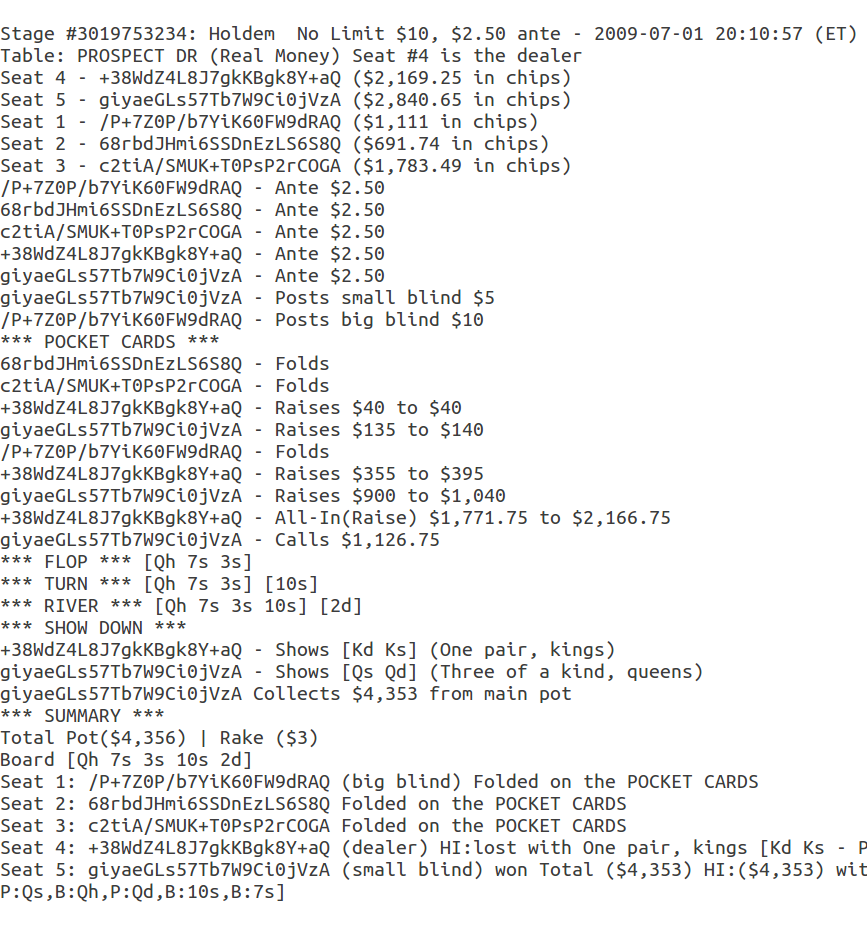
\includegraphics[width=.45\textwidth]{hand}
  		\caption{\textbf{Example hand.} One hand taken from the hand history files
  		we used in our project}
\end{figure}

The data contain information on about 15 million hands, and the obfuscated player
names were not a problem. In fact, working with anonymous data seems much better
with regard to research ethics. This data was fortunately perfect for our purposes,
to our great relief, and allowed us to proceed with our work.

\section*{Initial Investigations}
Our initial work involved doing some research into poker, the types of different
play styles, and a concrete metric we could compare our hands to.  We were
able to find some information about the primary differences in poker play styles,
as well as details about the value of different starting card combinations to the
player holding them. We thought we could use the play styles to help us interpret
any groupings among players that we might find in our analysis. We plotted the
starting hand values, in the hope that the resulting shape might be useful
as a comparison point for the shapes generated by actual players.

\begin{figure}[ht!]
		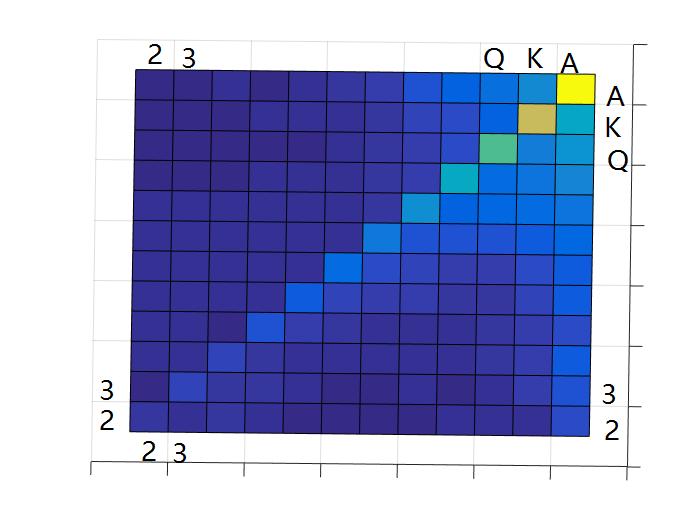
\includegraphics[width=.45\textwidth]{score}
  		\caption{\textbf{Heatmap of Poker Hand Values.} All possible differently 
  		valued starting Hold'Em hand combinations aligned in a grid, with 
  		their color indicating profitability (lighter is better)}
\end{figure}

We also
looked at academic literature to see if we could find work similar to ours which
we could apply. While we found academic papers on some aspects of poker, they
weren't topology related or particularly useful to our goals. We also found a
number of papers related to topology of games. Most of the topology papers dealt
with properties of special topological games, and of the remaining papers, there
were none which dealt with the topology of a player space or games with incomplete
information. So we needed to find our own techniques.

\section*{Hand Histories}
Before we could generate any results, we needed our data in a format that we could
work with. When we downloaded them, the hands were in a human-friendly format
that was not easy for programs to work with. Also, the files were grouped by
table stakes and by date and time, while we needed them to be grouped by player.

To deal with this, we wrote a small Perl script which parsed the raw hand
histories, retrieved the action of each player at all of their decision points,
and saved the information into individual files per player. This left us with
one file for each player, with each hand they played represented by one line of
numbers. We stored what action they took and how much money they invested at
each step, as well as how much they won or lost on each hand, and what their
cards were if that information was available.

In this format, it was easy for us to write code that could extract any information
we wanted about a given player, so that we could try a variety of different techniques
without needing to parse through seventy gigabytes of text files each time.

\section*{Player Shapes}
Once we had our data in a manageable form, we wanted to find some shape. We considered
quite a few options for how to look at the data, and ultimately decided on limiting
ourselves to considering the players' hole cards and their actions on the first
betting round. Our first reason for making this choice was that it just limited the
number of variables we would need to track, and reduced the dimension of our work.
In addition to that, the first round of betting has much less context, and so less
variability, than the later betting rounds. Actions in later rounds are very dependent
on actions in the first round, adding to the complexity of finding the usable information
we wanted. Also, we had already created a plot of the values of all the starting
hands in Texas Hold'em poker, which would be a nice metric of comparison as we tried
to see if our findings had a meaningful shape.


We created several more Perl scripts which could read the player files created by 
the first script and calculated the average amount of money they were willing 
to invest during the first betting round with each possible starting hand. We 
then used MATLAB to visualize these data in 2-dimensional and 3-dimensional
pictures, similar to the ones we created for the starting hand values. We partitioned
each player's hands into two random, independent groups so that we could check
them against each other to make sure that our methods were somewhat consistent.

\begin{figure}[ht!]
		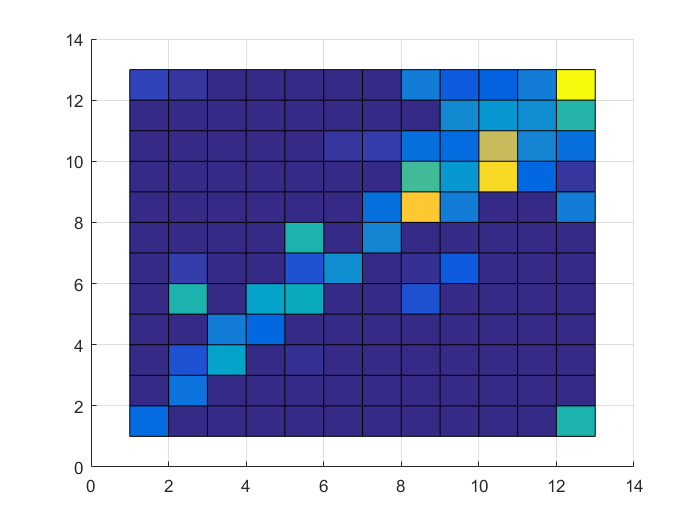
\includegraphics[width=.45\textwidth]{AfsU.png}
  		\caption{\textbf{Hands From a Winning Player.} This player's pattern has
  		a clear resemblance to the hand value chart shown above.}
\end{figure}

\begin{figure}[ht!]
		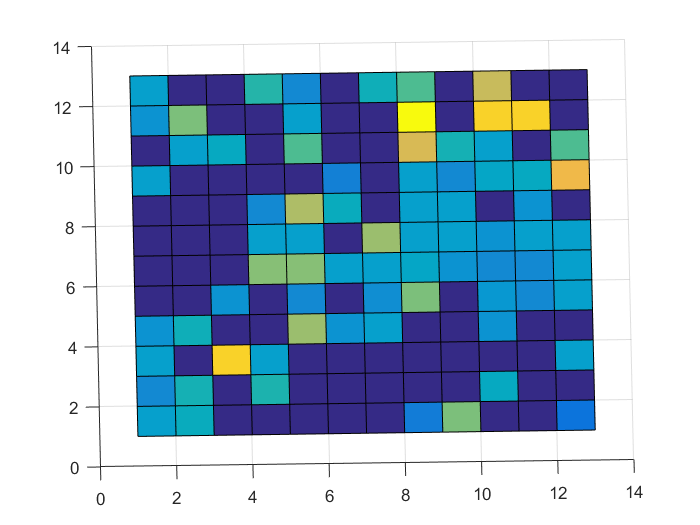
\includegraphics[width=.45\textwidth]{Ag6G2.png}
  		\caption{\textbf{Hands From a Losing Player.} The vaues in this chart
  		seem closer to a random sample than to the shape of hand values.}
\end{figure}

We also created a slightly different representation of the data, in which we
recorded one point for each time a player had a hand, rather than trying to
combine their play over all occurrences of a given hand. These data
created a point cloud, rather than a surface, which contained more
data but also had much more variation in it.

\begin{figure}[ht!]
		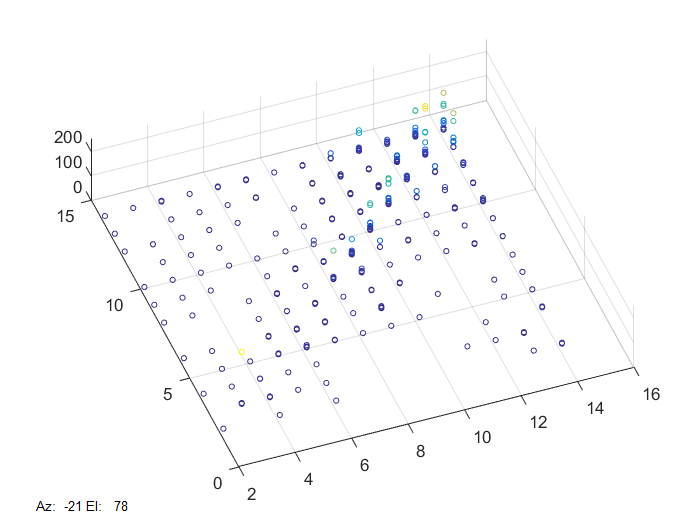
\includegraphics[width=.45\textwidth]{f1.png}
  		\caption{\textbf{Point Cloud Representation.} This point cloud version
  		is different from the above patterns, but still recognizable.}
\end{figure}

Looking at these charts, we were able to see clear patterns, and make some
conclusions about the players the charts had come from. Some of the charts which
were visually fairly similar to the starting hand value graphic belonged, as
expected, to the players who were winning at the highest rates. Also,
some of the shapes which bore little or no resemblance to the hand value shape
belonged to players with the heaviest losses. However, there was a great deal
of noise in the shapes, which we attributed mostly to the number of hands for each
player with hole card data available being limited.

\section*{Distance}
Our next step was to attempt to find a useful way to measure the distance
between the shapes generated by different players. Our
first attempt was to use a Hausdorff distance calculation package for R on our 
data. Unfortunately, we found that the distances calculated were not any closer
for our partitioned data than for shapes generated by completely different players.
This contradicted our principle that the techniques we use should return consistent
results.

We wrote a Java program which could read in the player shapes we had generated,
and store them as objects. We defined six different distance functions that we
thought might be useful for finding the distances. We had three basic types of
distance, and for each of them we ran two different versions, one in which each
point could be compared only to hands with the same starting cards, and another
which would compare across all hands in order to find the nearest points.

\begin{enumerate}
	\item The first distance was a sum of the distance between each point for
	one player and the nearest point in another player's set.
	\item The second distance was more of a Euclidean distance, with the square
	root of the sum of all nearest-point distances squared.
	\item The third distance was just the maximum of the distances between each
	point in one set and its nearest neighbor in another set.
\end{enumerate}

We had the Java program run batches of all of these distances on a sampling of
players, to see which gave the best performance.
We found our best results with the first distance option, on point clouds, with
comparison across different starting hands and setting a distance of sixteen
between adjacent squares.

 Unfortunately, the average distance between the shape of
two partitioned sets from one player was still only about 25\% closer than the
distance between shapes from two unrelated players. Even so, since we were seeing
some difference, we decided to put the player maps into a space, to see if we any
groupings could become apparent. We used a multi-dimentional scaling package for Java, 
and mapped each player to a single point in 2d and 3d spaces. Again, we thought
we could detect some patterns, but in these pictures they were even less distinct.

\begin{figure}[ht!]
		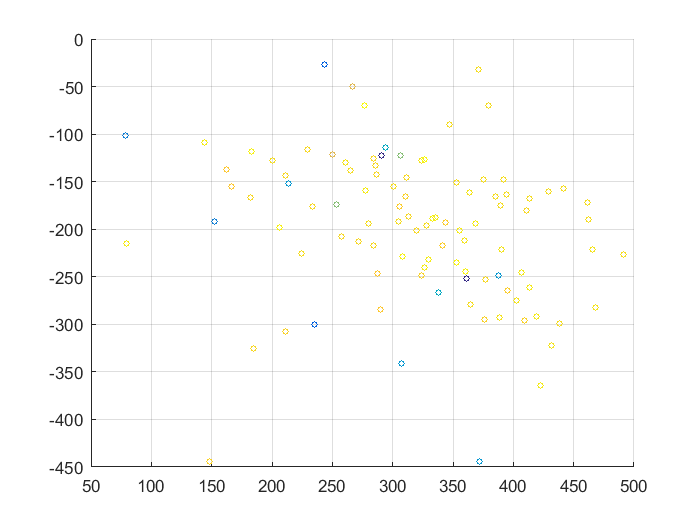
\includegraphics[width=.45\textwidth]{2dpart2_1.png}
  		\caption{\textbf{Player shapes put into a metric space.} The players are colored
  		by win rate, with the darkest dots losing the most. It seems that the
  		biggest losers tend to be far from the center.}
\end{figure}

\begin{figure}[ht!]
		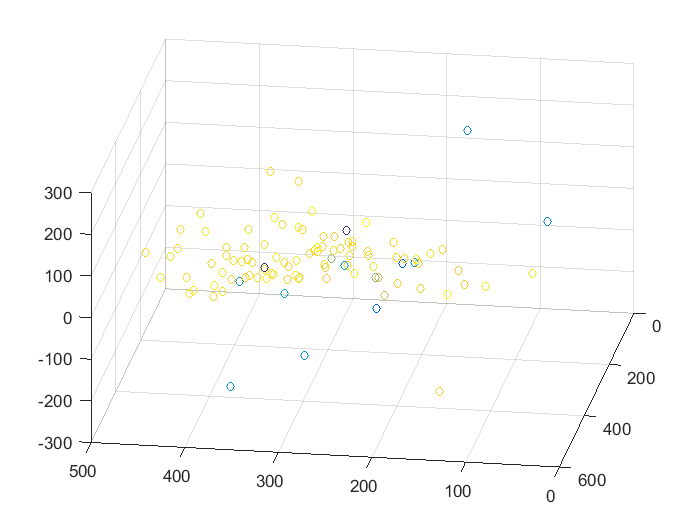
\includegraphics[width=.45\textwidth]{3dpart2_2.png}
  		\caption{\textbf{Players in a 3d metric space.} Again we see that most of the
  		players far out on some axis are significant losers.}
\end{figure}


\section*{Conclusion}
We tried several different techniques to analyze our poker hand history data,
but are somewhat disappointed with the results. We have been able to see
some interesting patterns and draw some conclusions, but we failed to find strong
conclusions or to have patterns which were apparent through computation. We feel
good about the work we did, and we think that a large part of our challenge had
to do more with the limitations of our data size, and the inherent difficulty of
working with a game of human decisions.

The fact that we can see a distinct difference between players, and that our
shapes show that winning players are more similar to each other than they are
to losing players our metric can be useful, but the
small magnitude of the difference makes it unhelpful for performing calculations
or coming to a better understanding of the data. We believe that if we had a larger
set of data with hole cards then we would be able to clean up some of the noise
and achieve more meaningful results.

In spite of the millions of hands of data which we had access to, and the fact
that there are tens of thousands of hands available for some players, our data
samples are not sufficient for the types of analysis we attempted. There
are two main issues at hand here. The first is that the inherent randomness of
poker means that many types of situations only come up very rarely, so data
about them converge very slowly. So slowly in fact that it is probable that
what is being measured will have changed before sufficient data are collected
to measure it.

However, we do believe that it would be well worthwhile to do further work in
this area. Given time, we could continue to work on creating a metric that does
not rely on hole cards, but only on the decisions that players make at each point.
That will increase the number of hands available for analysis significantly. Another
possibility is that we may convince one of the major poker websites, or hand
history sellers, to create a new and much larger set of poker hands. If it were
a poker site, they might even be able to furnish us with complete hole cards
for every player.

Although the results of our work are somewhat disappointing, we think our project
was a success. We think that
we the interesting patterns that we did find are worth the effort we put in, and more
importantly we learned a great deal in the process.

\newpage
~
\newpage
\begin{thebibliography}{9}

\bibitem{TopoIntro}
  Wikimedia Foundation,
  \emph{Topology},
  [Online] Available:
  https://en.wikipedia.org/wiki/Topology

\bibitem{Bowling15}
  Bowling, Michael, et al.,
  \emph{Heads-up limit hold'em poker is solved},
  Science,
  2015. 347: p 145-149.
  
\bibitem{Gale79}
  Gale, David,
  \emph{The Game of HEX and the Brouwer Fixed-Point Theorem},
  American Mathematiccal Monthly,
  1979. 86: p 818-827
	
\bibitem{Cao02}
  Cao, Jiling, et al.,
  \emph{Topological Properties Defined by Games and Their Applications},
  Topology \& Its Applications,
  2002. 123(1): p 47-55.
  
\bibitem{Kenderov93}
  Kenderov, P.S., and J.P.Revalski,
  \emph{Banach-Mazur Game and Generic Existence of Solutions to Optimization Problems},
  Proceedings of the American Mathematical Society,
  1993. 118: p 911-917.
  
\bibitem{TopoGame}
  Wikimedia Foundation,
  \emph{Topological Games},
  [Online]
  Available: http://en.wikipedia.org/wiki/Topological\_game.

\bibitem{BanachGame}
  Wikimedia Foundation,
  \emph{Banach-Mazur Game},
  [Online] Available:
  http://en.wikipedia.org/wiki/Banach-Mazur\_game.
  
\bibitem{PHHData}
  Outflopped.com,
  \emph{Obfuscated Datamined Hand Histories},
  [Online] Available:
  http://web.archive.org/web/20110205042259/
  http://www.outflopped.com/questions/286/
  obfuscated-datamined-hand-histories
  
\bibitem{MDSJ}
  Pich, Christian,
  \emph{MDSJ – Multidimensional Scaling for Java},
  [Online] Available: 
  http://algo.uni-konstanz.de/software/mdsj/

	
\end{thebibliography}

\end{document}
